% =====================================================================
% supplementary.tex -- supplementary material of the article.
% Published as received (not typeset by the journal), so it is compiled here
% to PDF. It refers to the article through xr, reading main.aux: build the
% article first.
%
% Build from this folder:
%   pdflatex main && bibtex main && pdflatex main && pdflatex main
%   pdflatex supplementary && bibtex supplementary && pdflatex supplementary && pdflatex supplementary
%
% Contents: S1 full table of cases (generated by maps/paper_tables.py);
% S2 application to three field conveyors (figure and table generated by the
% code); S3 drive on the return strand and initial crawl; S4 illustrative conveyors of the
% verification; S5 further details moved from the article. No statement of the
% article rests only on this material.
% Numbers are macros of paper_numbers.tex, as in the article.
% =====================================================================
\documentclass[a4paper,11pt]{article}
\usepackage[margin=25mm]{geometry}
\usepackage[T1]{fontenc}
\usepackage[utf8]{inputenc}
\usepackage{lmodern}
\usepackage{microtype}
\usepackage{amsmath,amssymb}
\usepackage[separate-uncertainty=true,per-mode=symbol]{siunitx}
\usepackage{array,booktabs,threeparttable}
\usepackage{graphicx}
\graphicspath{{../maps/figures/paper/}{../validation/figures/}{figures/}}
\usepackage{rotating}
\usepackage[numbers,sort&compress]{natbib}
\usepackage{xcolor}
% Cross-references to the article (labels read from main.aux). The prefix A-
% keeps the article's labels and reference numbers apart from those of this
% document: \ref{A-sec:results} is Section 5 of the article, and the citations
% here are numbered in this document's own reference list.
\usepackage{xr}
\externaldocument[A-]{main}

% The wide generated tables open a widetable float: a landscape page here.
\newenvironment{widetable}[1][t]{\begin{sidewaystable}}{\end{sidewaystable}}

% Numbering S1, S2, ... for sections, figures, tables and equations.
\renewcommand{\thesection}{S\arabic{section}}
\renewcommand{\thefigure}{S\arabic{figure}}
\renewcommand{\thetable}{S\arabic{table}}
\renewcommand{\theequation}{S\arabic{equation}}

% =====================================================================
% macros.tex -- notation and editing macros of the manuscript.
% Keep this file small: a macro is worth it only if a symbol appears
% many times or its typesetting may change in one place.
% =====================================================================

% ---- Editing aids (remove or empty \TODO before submission) ---------
\newcommand{\TODO}[1]{\textcolor{red}{[#1]}}
\newcommand{\NOTE}[1]{\textcolor{blue}{[#1]}}

% ---- Generic operators ----------------------------------------------
\newcommand{\dd}{\mathrm{d}}                    % differential
\newcommand{\ee}{\mathrm{e}}                    % Euler's number
\newcommand{\ii}{\mathrm{i}}                    % imaginary unit
\newcommand{\jump}[1]{[\![#1]\!]}               % jump across a point
\newcommand{\T}{\mathsf{T}}                     % transpose
\newcommand{\mat}[1]{\mathbf{#1}}               % matrices and vectors

% ---- Notation decided in step 6.2 (see sections/notation.tex) -------
% Periods and transit times are lower-case t (dimensional) and tau
% (dimensionless, units of L/c_r), like t_a and tau_a; T is kept for
% tensions (T_0, T_d, T_t and the drive tensions T_1, T_2 of DIN 22101).
% Changing one of these macros here changes it everywhere.
\newcommand{\Mtu}{M}                 % take-up mass referred to its pulley
\newcommand{\nstr}{n}                % belt strands that carry the take-up pulley
\newcommand{\Tt}{T_t}                % static belt tension at the take-up
\newcommand{\Wret}{W_r}              % weight of the return strand, g mu_r L (not \Wr: txfonts and others define it)
\newcommand{\mw}{m'}                % line density that contributes to weight (DIN 22101 m')
\newcommand{\egrip}{\ee^{\mu\theta}}  % drive factor; E is reserved for Young's modulus
\newcommand{\tper}[1]{t_{#1}}        % natural period of mode #1 (s)
\newcommand{\tauper}[1]{\tau_{#1}}   % the same period in units of L/c_r
\newcommand{\tauB}{\tau_B}           % transit time of strand B, 1 - xi + gamma (units of L/c_r)
\newcommand{\betafive}{\beta_5}      % take-up mass threshold (5 % period change)

% ---- Numbers from the code ------------------------------------------
% paper_numbers.tex defines one macro per number quoted in the text,
% named \Num<Topic><Quantity>, e.g. \NumHarrisonPeriod. Units stay in
% the text: \qty{\NumHarrisonPeriod}{\second}.

% =====================================================================
% paper_numbers.tex -- GENERATED by maps/paper_numbers.py; do not edit.
% Regenerate with:  python maps/paper_numbers.py   (from the repository root)
% One macro per number quoted in the text, already rounded, without its
% unit. Use them as \qty{\NumHarrisonSlowModel}{\second}, \num{\NumX} or
% plain \NumX. Percentages are in per cent.
% =====================================================================


% ---- Take-up mass against its threshold (paper_figures.case_margins, case table)
\newcommand{\NumLongBetaMax}{0.205}  % largest beta, conveyors of 1 km or longer
\newcommand{\NumLongMarginMin}{3.7}  % smallest beta_5(B1)/beta, alpha = 1
\newcommand{\NumLongMarginMinLow}{2.8}  % the same, lowest coupling
\newcommand{\NumLongShiftMax}{1.2}  % largest lengthening of t_1 (%), alpha = 1
\newcommand{\NumLongShiftMaxLow}{1.8}  % the same, lowest coupling (%)
\newcommand{\NumShiftH}{0.15}  % H: lengthening of t_1 by the take-up mass (%), alpha = 1
\newcommand{\NumShiftHLow}{0.15}  % H: the same at the lowest coupling (%)
\newcommand{\NumBetaRatioH}{0.03}  % H: beta / beta_5(B1)
\newcommand{\NumShiftS}{1.07}  % S: lengthening of t_1 by the take-up mass (%), alpha = 1
\newcommand{\NumShiftSLow}{1.23}  % S: the same at the lowest coupling (%)
\newcommand{\NumBetaRatioS}{0.22}  % S: beta / beta_5(B1)
\newcommand{\NumShiftSt}{1.23}  % St: lengthening of t_1 by the take-up mass (%), alpha = 1
\newcommand{\NumShiftStLow}{1.61}  % St: the same at the lowest coupling (%)
\newcommand{\NumBetaRatioSt}{0.27}  % St: beta / beta_5(B1)
\newcommand{\NumShiftG}{0.03}  % G: lengthening of t_1 by the take-up mass (%), alpha = 1
\newcommand{\NumShiftGLow}{0.04}  % G: the same at the lowest coupling (%)
\newcommand{\NumBetaRatioG}{0.01}  % G: beta / beta_5(B1)
\newcommand{\NumShiftLL}{0.54}  % LL: lengthening of t_1 by the take-up mass (%), alpha = 1
\newcommand{\NumShiftLLLow}{0.66}  % LL: the same at the lowest coupling (%)
\newcommand{\NumBetaRatioLL}{0.11}  % LL: beta / beta_5(B1)
\newcommand{\NumShiftSM}{0.85}  % SM: lengthening of t_1 by the take-up mass (%), alpha = 1
\newcommand{\NumShiftSMLow}{1.44}  % SM: the same at the lowest coupling (%)
\newcommand{\NumBetaRatioSM}{0.17}  % SM: beta / beta_5(B1)
\newcommand{\NumShiftLo}{0.73}  % Lo: lengthening of t_1 by the take-up mass (%), alpha = 1
\newcommand{\NumShiftLoLow}{1.15}  % Lo: the same at the lowest coupling (%)
\newcommand{\NumBetaRatioLo}{0.15}  % Lo: beta / beta_5(B1)
\newcommand{\NumShiftPa}{1.19}  % Pa: lengthening of t_1 by the take-up mass (%), alpha = 1
\newcommand{\NumShiftPaLow}{1.78}  % Pa: the same at the lowest coupling (%)
\newcommand{\NumBetaRatioPa}{0.24}  % Pa: beta / beta_5(B1)
\newcommand{\NumShiftSi}{0.13}  % Si: lengthening of t_1 by the take-up mass (%), alpha = 1
\newcommand{\NumShiftSiLow}{0.18}  % Si: the same at the lowest coupling (%)
\newcommand{\NumBetaRatioSi}{0.03}  % Si: beta / beta_5(B1)
\newcommand{\NumLongTtWrMin}{0.01}  % T_t/W_r, conveyors of 1 km or longer
\newcommand{\NumLongTtWrMax}{0.10}
\newcommand{\NumLongBetaRatioMin}{0.01}  % beta / beta_5(B1), conveyors of 1 km or longer (G: beta from its counterweight mass)
\newcommand{\NumLongBetaRatioMax}{0.27}

% ---- Short conveyors where beta starts to matter (WR, Su)
\newcommand{\NumWRBeta}{0.88}  % Wheatley and Rubel, 275 m
\newcommand{\NumWRRatioMin}{0.56}  % beta/beta_5(B1) over the take-up positions
\newcommand{\NumWRRatioMax}{0.58}
\newcommand{\NumWRRatioLowMin}{0.95}  % the same at alpha = 0.8
\newcommand{\NumWRRatioLowMax}{1.02}
\newcommand{\NumWRShiftLowMin}{4.7}  % lengthening of t_1 at alpha = 0.8 (%)
\newcommand{\NumWRShiftLowMax}{5.1}
\newcommand{\NumSuBeta}{0.64}  % Surtees, 805 m, design 2
\newcommand{\NumSuRatio}{0.42}  % beta/beta_5(B1)
\newcommand{\NumSuRatioLow}{0.66}  % the same at alpha = 0.8
\newcommand{\NumSuShift}{2.1}  % lengthening of t_1 (%)
\newcommand{\NumSuShiftLow}{3.3}  % the same at alpha = 0.8 (%)
\newcommand{\NumWRBLength}{247}  % Wheatley and Rubel, conveyor B: length (m)
\newcommand{\NumWRBBeta}{1.30}
\newcommand{\NumWRBRatio}{0.84}  % beta / beta_5(B1)
\newcommand{\NumWRCLength}{91}  % Wheatley and Rubel, conveyor C: length (m)
\newcommand{\NumWRCBeta}{2.13}
\newcommand{\NumWRCRatio}{1.38}  % beta / beta_5(B1)

% ---- Belt speed over wave speed, assumption (A4)
\newcommand{\NumSpeedRatioMin}{0.003}  % smallest V / c_c, cases other than Lo
\newcommand{\NumSpeedRatioMax}{0.01}  % largest V / c_c, cases other than Lo
\newcommand{\NumSpeedRatioLo}{0.03}  % V / c_c of Lodewijks' fabric belt, loaded

% ---- Frequencies and participation (fig_modal; head drive, beta -> 0)
\newcommand{\NumModalTauMin}{4.01}  % tau_1 = t_1 c_r / L over the map
\newcommand{\NumModalTauMax}{13.42}
\newcommand{\NumModalFourTransitMin}{0.838}  % tau_1 / (4 tau_B), lower bound over the map
\newcommand{\NumModalFourTransitOver}{19}  % largest overestimate of the four-transit rule (%)
\newcommand{\NumModalParticipationMin}{0.41}  % effective-mass fraction of the fundamental
\newcommand{\NumModalParticipationMax}{0.81}
\newcommand{\NumModalHatched}{7}  % share of the (xi, gamma) plane where beta = 0.1 changes it by > 5 % (%)
\newcommand{\NumModalHatchedMedian}{1.5}  % median change of the fundamental's participation with beta = 0.1 (%)
\newcommand{\NumModalParticipationFormulaErr}{3.1}  % largest overestimate of F_1 ~ (8/pi^2)(1 - xi + gamma^2)/(1 + gamma^2) over the map (%)
\newcommand{\NumHeadTailRatioGammaOne}{2.00}  % t_1 with the take-up at the head over t_1 at the tail, gamma = 1
\newcommand{\NumHeadTailRatioGammaOneFive}{1.49}  % t_1 with the take-up at the head over t_1 at the tail, gamma = 1.5
\newcommand{\NumHeadTailRatioGammaTwo}{1.28}  % t_1 with the take-up at the head over t_1 at the tail, gamma = 2
\newcommand{\NumHeadTailRatioGammaThree}{1.12}  % t_1 with the take-up at the head over t_1 at the tail, gamma = 3
\newcommand{\NumIntermediateRatioMax}{1.38}  % tau_1/(4 tau_B) with an intermediate drive, gamma <= 3
\newcommand{\NumIntermediateOverMax}{38}  % the same as an excess over four transits (%)
\newcommand{\NumNCRatio}{1.17}  % Nordell and Ciozda: tau_1/(4 tau_B)
\newcommand{\NumNCPeriod}{27.5}  % Nordell and Ciozda: t_1 (s), beta -> 0
\newcommand{\NumNCPeriodHead}{19.8}  % the same strands with a head drive (s)
\newcommand{\NumNCIncrease}{39}  % (%)
\newcommand{\NumNCFourTransit}{23.4}  % Nordell and Ciozda: four transits of strand B (s)
\newcommand{\NumNCRatioHead}{0.84}  % the same strands with a head drive: tau_1/(4 tau_B)
\newcommand{\NumSuFourTransit}{0.952}  % Surtees: tau_1/(4 tau_B), beta -> 0
\newcommand{\NumSuFourTransitLow}{0.939}  % the same at alpha = 0.8

% ---- Song et al. (2012): take-up next to the head drive against the tail
\newcommand{\NumSongPeriodHead}{40.4}  % t_1 (s), beta from the take-up tension (case table)
\newcommand{\NumSongPeriodTail}{29.0}
\newcommand{\NumSongPeriodHeadLight}{40.0}  % t_1 (s), beta -> 0, as Song et al. modelled it; quoted in the text
\newcommand{\NumSongPeriodTailLight}{28.6}
\newcommand{\NumSongBetaMass}{0.017}  % beta of their 4500 kg counterweight on two strands
\newcommand{\NumSongShiftMass}{0.15}  % lengthening of t_1 at the tail with that beta (%)
\newcommand{\NumSongFourTransit}{45.8}  % four transits of strand B, take-up at the head (s)
\newcommand{\NumSongFourTransitRatio}{0.873}  % t_1 / four transits, take-up at the head, beta -> 0

% ---- Take-up mass threshold (fig_beta)
\newcommand{\NumBetaFiveBOneMin}{0.11}  % beta_5 of the fundamental (B1) over the map
\newcommand{\NumBetaFiveBOneMax}{1.66}
\newcommand{\NumBetaFiveBOneMedian}{0.76}
\newcommand{\NumBetaFiveBTwoMedian}{0.39}
\newcommand{\NumBetaFiveMinGammaOneFour}{0.33}  % smallest beta_5(B1) for gamma >= 1.4, any take-up position (at the tail)
\newcommand{\NumBetaFiveMinNearDrive}{0.49}  % smallest beta_5(B1), gamma >= 1.4, xi <= 0.1: the rule T_t <~ W_r/4 (n = 2) is stated for a take-up near the drive
\newcommand{\NumRuleGammaAnyPosition}{1.7}  % gamma above which beta_5(B1) >= 0.5 for every take-up position (grid 0.025)
\newcommand{\NumSinglePoleCoefficient}{0.41}  % beta_5 ~ 0.41 m~ (one pole)
\newcommand{\NumBetaFiveAOneSlope}{0.205}  % beta_5(A1) ~ 0.205 xi (uniform strand)
\newcommand{\NumStAOneShift}{3.2}  % St (take-up at the tail): lengthening of A1 by the take-up mass (%)
\newcommand{\NumAOneStartRatioMin}{3.3}  % smallest tau_a / tau_A1 of the published starts with the take-up at the tail (Lo)

% ---- Universal start-up curve (fig_startup; sine profile unless stated)
\newcommand{\NumStartPeakMax}{1.590}  % largest amplification D
\newcommand{\NumStartPeakAt}{0.87}  % at tau_a / tau_s
\newcommand{\NumStartDOne}{1.574}  % D at tau_a / tau_s = 1 (exact ratio)
\newcommand{\NumStartDTwo}{1.206}  % D at tau_a / tau_s = 2 (exact ratio)
\newcommand{\NumStartDThree}{1.130}  % D at tau_a / tau_s = 3 (exact ratio)
\newcommand{\NumStartDFive}{1.077}  % D at tau_a / tau_s = 5 (exact ratio)
\newcommand{\NumStartDTen}{1.039}  % D at tau_a / tau_s = 10 (exact ratio)
\newcommand{\NumStartTriangularMax}{1.333}
\newcommand{\NumStartParabolicMax}{1.621}
\newcommand{\NumStartTriangularExcess}{26}  % triangular over sine per unit mean acceleration, tau_a = 5 tau_s (%)
\newcommand{\NumStartDampTwo}{1.549}  % largest D with zeta_1 = 0.02
\newcommand{\NumStartDampFive}{1.496}  % largest D with zeta_1 = 0.05
\newcommand{\NumStartDampTen}{1.425}  % largest D with zeta_1 = 0.1
\newcommand{\NumStartTravelMax}{1.80}  % take-up travel over quasi-static, largest
\newcommand{\NumStartResOne}{1.273}  % resistances with phi = V/V_inf, tau_a / tau_s = 1 (exact ratio)
\newcommand{\NumStartResTwo}{1.055}  % resistances with phi = V/V_inf, tau_a / tau_s = 2 (exact ratio)
\newcommand{\NumStartResFive}{1.008}  % resistances with phi = V/V_inf, tau_a / tau_s = 5 (exact ratio)
\newcommand{\NumCollapseEntryEight}{1.7}  % loop against the strand curve at the drive entry, tau_a >= 0.8 tau_1 (%)
\newcommand{\NumCollapseExitEight}{0.3}  % the same at the exit (%)
\newcommand{\NumCollapseEntryFive}{5.6}  % loop against the strand curve at the drive entry, tau_a >= 0.5 tau_1 (%)
\newcommand{\NumCollapseExitFive}{1.0}  % the same at the exit (%)
\newcommand{\NumCollapseEntryOne}{1.1}  % loop against the strand curve at the drive entry, tau_a >= 1 tau_1 (%)
\newcommand{\NumCollapseExitOne}{0.3}  % the same at the exit (%)
\newcommand{\NumCollapseFastMax}{63}  % entry, fastest start (tau_a = 0.2 tau_1), gamma != 1 (%)
\newcommand{\NumCollapseUniformMax}{0.6}  % entry, gamma = 1 (uniform strand B), any start time (%)
\newcommand{\NumPracticeLo}{1.05}  % Lo: published start time over its t_1
\newcommand{\NumPracticeLL}{1.49}  % LL: published start time over its t_1
\newcommand{\NumPracticeG}{2.43}  % G: published start time over its t_1
\newcommand{\NumPracticeSu}{4.11}  % Su: published start time over its t_1
\newcommand{\NumPracticeS}{7.43}  % S: published start time over its t_1
\newcommand{\NumPracticeSi}{11.81}  % Si: published start time over its t_1
\newcommand{\NumPracticeSTail}{10.36}  % S: 300 s over t_1 at the tail, where simulated
\newcommand{\NumPracticeLLAccel}{1.28}  % LL: 60 s after the 10 s of motor switching, over t_1

% ---- Initial crawl (fig_crawl; rho = 1, 5 and zeta_1 = 0.01, 0.1)
\newcommand{\NumCrawlAbruptMin}{1.17}  % entry peak / (R + m a_m), abrupt onset
\newcommand{\NumCrawlAbruptMax}{1.66}
\newcommand{\NumCrawlRampHalfMin}{1.07}  % ramp of 0.5 tau_1
\newcommand{\NumCrawlRampHalfMax}{1.36}
\newcommand{\NumCrawlRampOneMin}{1.01}  % ramp of one tau_1
\newcommand{\NumCrawlRampOneMax}{1.07}
\newcommand{\NumCrawlTravelAbruptMin}{1.2}  % take-up travel / quasi-static
\newcommand{\NumCrawlTravelAbruptMax}{1.8}
\newcommand{\NumCrawlTravelRampOneMax}{1.09}
\newcommand{\NumCrawlHoldDampedZero}{1.17}  % rho = 1, zeta_1 = 0.1: entry peak after a hold of 0 tau_1
\newcommand{\NumCrawlHoldDampedOne}{1.09}  % rho = 1, zeta_1 = 0.1: entry peak after a hold of 1 tau_1
\newcommand{\NumCrawlHoldDampedTwo}{1.05}  % rho = 1, zeta_1 = 0.1: entry peak after a hold of 2 tau_1

% ---- Validity conditions (fig_validity; gamma = 2, rho = 1 in (c) and (d))
\newcommand{\NumReboundMax}{1.44}  % rebound of strand B, no resistances, / (m_B a_m)
\newcommand{\NumValidityExitMax}{0.14}  % required T_2 at the exit / (m_belt a_m)
\newcommand{\NumValidityGripThreeMin}{0.88}  % grip with e^{mu theta} = 3
\newcommand{\NumValidityGripThreeMax}{1.28}
\newcommand{\NumValidityGripSixteenMin}{0.12}  % grip with e^{mu theta} = 16
\newcommand{\NumValidityGripSixteenMax}{0.29}
\newcommand{\NumTightMin}{1.80}  % take-up tension on the tight side / (m_belt a_m)
\newcommand{\NumTightMax}{2.08}
\newcommand{\NumSlackMin}{0.14}  % the same on the slack side
\newcommand{\NumSlackMax}{0.27}

% ---- Take-up kinematics (maps/validity.kinematics; 1 <= gamma <= 3, any xi, sine, beta -> 0)
\newcommand{\NumTakeupAccEnvelope}{2.5}  % largest |y''| / a_m, belt side, any start time
\newcommand{\NumTakeupVelFast}{1.75}  % largest |y'| / V_inf, tau_a = 0.01 tau_1
\newcommand{\NumTakeupVelFifth}{1.14}  % largest |y'| / V_inf, tau_a >= 0.2 tau_1
\newcommand{\NumTakeupVelOne}{0.30}  % largest |y'| / V_inf, tau_a >= 1 tau_1
\newcommand{\NumTakeupVelOneFour}{0.08}  % largest |y'| / V_inf, tau_a >= 1.4 tau_1
\newcommand{\NumTakeupAccSlow}{0.5}  % largest |y''| / a_m, tau_a >= 1.4 tau_1

% ---- Application to field conveyors (fig_applications, table_applications)
\newcommand{\NumLoTt}{21.3}  % Lodewijks: take-up tension of the case (kN)
\newcommand{\NumLoTtReq}{51.5}  % required for the 30 s start, real position (kN)
\newcommand{\NumLoTtReqTail}{56.1}  % the same, take-up at the tail (kN)
\newcommand{\NumLoTtReqRigid}{35.2}  % the same with a rigid belt, same loads (kN)
\newcommand{\NumLoDynamicIncrement}{46}  % increase of the required T_t by the belt dynamics (%)
\newcommand{\NumLoShortest}{101}  % shortest admissible sine start, real position (s)
\newcommand{\NumLoShortestOverPeriod}{3.56}  % the same over t_1
\newcommand{\NumLoShortestRigid}{85}  % the same with a rigid belt, same loads (s)
\newcommand{\NumLoGammaLow}{2.15}  % Lo: gamma at the weakest coupling of the material
\newcommand{\NumLoPeriodLow}{24.2}  % Lo: t_1 at the weakest coupling (s)
\newcommand{\NumLoPeriod}{28.5}  % Lo: t_1 at full coupling, real position (s)
\newcommand{\NumLoPracticeLow}{1.24}  % Lo: 30 s start over t_1 at the weakest coupling
\newcommand{\NumLoRuleMin}{57}  % Lo: 2 t_1 (s)
\newcommand{\NumLoRuleMax}{85}  % Lo: 3 t_1 (s)
\newcommand{\NumLoRuleMinLow}{48}  % Lo: 2 t_1 at the weakest coupling (s)
\newcommand{\NumLoPeriodChange}{12}  % t_1, real to tail (%)
\newcommand{\NumLoXiLimit}{0.82}  % beyond this take-up position no start is admissible (running grip fails)
\newcommand{\NumLoGripRatioMin}{4.2}  % max T_entry/T_exit in the 30 s starts of Table 8.7
\newcommand{\NumLoGripRatioMax}{6.1}
\newcommand{\NumLoGripFactor}{3.0}  % e^{mu theta} of his drive
\newcommand{\NumLoSineTtFactor}{2.4}  % sine 30 s start: T_t needed for grip over his T_t
\newcommand{\NumSMTtReq}{60}  % Suchorab-Matuszewska: required T_t, real position (kN)
\newcommand{\NumSMTtReqTail}{22}  % the same at the tail (kN)
\newcommand{\NumSMTt}{140}  % take-up tension of the case (kN)
\newcommand{\NumSMShortest}{13}  % shortest admissible start (s)
\newcommand{\NumSMPeriodChange}{20}  % t_1, real to tail (%)
\newcommand{\NumSMReferenceStart}{40.8}  % reference start 3 t_1 (s)
\newcommand{\NumSuTtReq}{19.8}  % Surtees: required T_t after the drive (kN)
\newcommand{\NumSuTtReqTight}{234}  % the same on the tight side (kN)
\newcommand{\NumSuTightFactor}{12}  % tight over slack side
\newcommand{\NumSuShortest}{7.4}  % shortest admissible start (s)
\newcommand{\NumSuExitTight}{-114}  % lowest exit tension on the tight side (kN)
\newcommand{\NumSMShortestOverPeriod}{1.0}  % SM: shortest start over t_1
\newcommand{\NumSuShortestOverPeriod}{1.2}  % Su: shortest start over t_1
\newcommand{\NumSMTtReqMax}{83}  % SM: largest required T_t along the return (kN)
\newcommand{\NumSuTtReqBest}{18.1}  % Su: smallest required T_t along the return, slack side (kN)
\newcommand{\NumAppAccelMarginMin}{38}  % condition 2 (take-up follows the belt): smallest margin in the application runs
\newcommand{\NumSMGripFactor}{16.4}  % SM: e^{mu theta} of the tandem drive
\newcommand{\NumSuGripFactor}{11.5}  % Su: e^{mu theta} of the drive
\newcommand{\NumSuDrivePos}{0.197}  % Su: drive position sigma_d/L from the head

% ---- Validation: Harrison (1983, 1985b) (validation/harrison_case.py)
\newcommand{\NumHarrisonSlowMeas}{24.9}  % measured slow period (s), our read-out of Fig. 5e
\newcommand{\NumHarrisonSlowModel}{28.4}  % model (s): n = 4, gamma = 0.97, xi = 0.005
\newcommand{\NumHarrisonSlowExcess}{14}  % (%)
\newcommand{\NumHarrisonSlowModelMin}{27.6}  % model over the measured gamma band (s)
\newcommand{\NumHarrisonSlowModelMax}{29.1}
\newcommand{\NumHarrisonSecondMin}{9.3}  % second period of the model (s)
\newcommand{\NumHarrisonSecondMax}{9.4}
\newcommand{\NumHarrisonWaveMeas}{7.3}  % measured ripple (s), Fig. 5c
\newcommand{\NumHarrisonEmbeddedMax}{14.1}  % embedded-mass model, largest fundamental for xi <= 0.2 (s)
\newcommand{\NumHarrisonBetaMin}{0.012}  % beta = 4M/(n^2 mu_r L), n = 4, rho = 79 and 39 kg/m
\newcommand{\NumHarrisonBetaMax}{0.024}
\newcommand{\NumHarrisonMuRLow}{40}  % mu_r of the return strand for rho = 39 kg/m (kg/m)
\newcommand{\NumHarrisonMuRHigh}{81}  % the same for rho = 79 kg/m (kg/m)
\newcommand{\NumHarrisonGammaMeas}{0.97}  % gamma measured on the empty belt (1985b)
\newcommand{\NumHarrisonGammaMeasMin}{0.90}
\newcommand{\NumHarrisonGammaMeasMax}{1.06}
\newcommand{\NumHarrisonStillMeas}{7.6}  % return belt still after the start (s), measured
\newcommand{\NumHarrisonTransit}{7.0}  % model: time until the wave returns (s)
\newcommand{\NumHarrisonStillSpeed}{0.007}  % model: largest belt speed there meanwhile (m/s)
\newcommand{\NumHarrisonCarriageModel}{2.0}  % model: carriage travel at 7 s (m)
\newcommand{\NumHarrisonCarriageMeas}{2}  % measured carriage travel, about (m)
\newcommand{\NumHarrisonStoredMax}{10}  % model: belt stored in the loop (m)
\newcommand{\NumHarrisonStoredRunMin}{7}  % belt stored by the running resistances, 900 kW on the empty belt, rho = 79 kg/m (m)
\newcommand{\NumHarrisonStoredRunMax}{15}  % the same, rho = 39 kg/m (m)
\newcommand{\NumHarrisonStoredMeas}{24}  % belt released by the loop at start-up, 1985b text (m)
\newcommand{\NumHarrisonTransmissionMin}{0.02}  % |t| through the take-up at 7 s
\newcommand{\NumHarrisonTransmissionMax}{0.04}

% ---- Validation: Harrison, drive without speed control (Section 3.6)
\newcommand{\NumHarrisonFreeDriveSlow}{14.2}  % free drive (m_d -> 0): slow period (s)
\newcommand{\NumHarrisonFreeDriveSecond}{7.0}  % free drive: second period (s), the loop transit
\newcommand{\NumHarrisonDriveMassMeas}{4.8}  % m_d that alone gives the measured slow period
\newcommand{\NumHarrisonDriveMassBeltRatio}{2.5}  % that reduced drive mass over the mass of the whole belt
\newcommand{\NumHarrisonDriveMassSecond}{9.2}  % second period with that m_d (s)
\newcommand{\NumHarrisonRunForce}{243}  % running force 900 kW / 3.7 m/s (kN)
\newcommand{\NumHarrisonSlipNatural}{3}  % assumed slip, natural characteristic (%)
\newcommand{\NumHarrisonSlipSoftMin}{20}  % assumed slip, rotor resistance in circuit (%)
\newcommand{\NumHarrisonSlipSoftMax}{30}
\newcommand{\NumHarrisonDashpotNatural}{19}  % c_hat on the natural characteristic
\newcommand{\NumHarrisonDashpotNaturalChange}{0.4}  % largest change of the slow period with it, m_d = 0.1-3 (%)
\newcommand{\NumHarrisonDashpotSoftMin}{1.9}  % c_hat with rotor resistance in circuit
\newcommand{\NumHarrisonDashpotSoftMax}{2.8}
\newcommand{\NumHarrisonSoftSlowMin}{23.9}  % slow period with it, m_d = 1-3 (s)
\newcommand{\NumHarrisonSoftSlowMax}{26.4}
\newcommand{\NumHarrisonSoftZetaMin}{0.08}  % its damping ratio
\newcommand{\NumHarrisonSoftZetaMax}{0.23}
\newcommand{\NumHarrisonSoftSecondMin}{8.9}  % second period with it (s)
\newcommand{\NumHarrisonSoftSecondMax}{9.1}
\newcommand{\NumHarrisonDriveMassMin}{0.1}  % range of m_d tried
\newcommand{\NumHarrisonDriveMassMax}{3}

% ---- Validation: Nordell and Ciozda (1984), arrival times (case geometry, two wave speeds)
\newcommand{\NumNCArrivalB}{3.74}  % wave from the drive to point B (s); measured 3.72
\newcommand{\NumNCArrivalC}{5.86}  % wave from the drive to the take-up, point C (s); measured 5.86
\newcommand{\NumNCArrivalBShort}{2.18}  % front from the drive to point B through the take-up and the tail (s); absent in the record (Nordell 1987, Fig. 7)
\newcommand{\NumNCArrivalBMeas}{3.72}  % measured (their Fig. 10)
\newcommand{\NumNCArrivalCMeas}{5.86}  % measured (their Fig. 11)
\newcommand{\NumNCSpeedReturn}{1450}  % their wave speed on the empty return strand (m/s)
\newcommand{\NumNCSpeedCarry}{590}  % their wave speed on the loaded carry strand (m/s)

% ---- Validation: Muja P2 (cdi1998), published values
\newcommand{\NumMujaLength}{6.1}  % km
\newcommand{\NumMujaTime}{3.1}  % wave travel time in an emergency stop, empty belt (s)
\newcommand{\NumMujaSpeedMeas}{1968}  % (m/s)
\newcommand{\NumMujaSpeedCalc}{1985}  % from E and density (m/s)
\newcommand{\NumMujaSpeedDiff}{0.9}  % (%)

% ---- Cross-comparison: Song et al. (2012) (validation/song_case.py)
\newcommand{\NumSongCcModel}{995.6}  % carry wave speed from their data (m/s)
\newcommand{\NumSongCcPub}{995.6}  % published
\newcommand{\NumSongCrModel}{1658.7}  % return wave speed from their data (m/s)
\newcommand{\NumSongCrPub}{1668.7}  % published
\newcommand{\NumSongFRunModel}{224}  % running drive force from their resistance law (kN)
\newcommand{\NumSongFRunPub}{226.8}  % published (kN)
\newcommand{\NumSongFRunDiff}{1}  % (%)
\newcommand{\NumSongTtPub}{173}  % published tension at the tail take-up (kN)
\newcommand{\NumSongTtMass}{22}  % what 4500 kg hold on two strands (kN)
\newcommand{\NumSongTravelPub}{2.81}  % published steady take-up travel (m)
\newcommand{\NumSongTravelTensions}{1.8}  % take-up travel implied by their own running tensions (m)

% ---- Cross-comparison: Lodewijks (1996) ch. 8 (validation/data/lodewijks_case.json)
\newcommand{\NumLodewijksPeakDevMin}{-18}  % peak strain, model / his - 1 (%)
\newcommand{\NumLodewijksPeakDevMax}{0}
\newcommand{\NumLodewijksPeriodMeas}{18.3}  % his oscillation period (s)
\newcommand{\NumLodewijksPeriodModel}{28.5}  % ours (s)
\newcommand{\NumLodewijksLinearGap}{1}  % model: offset vs plain linear ramp, peak strain difference (%)
\newcommand{\NumLodewijksLinearGapHis}{3}  % the same in his Table 8.7 (%)
\newcommand{\NumLodewijksTravelMeanHis}{3.6}  % mean take-up travel after his 30 s start (m), our fit of his Fig. 8.42
\newcommand{\NumLodewijksTravelSweepHis}{2.0}  % his largest take-up travel for a 50 s start (m), Fig. 8.46
\newcommand{\NumLodewijksTravelMeanModel}{2.6}  % ours after the 30 s start (m)
\newcommand{\NumLodewijksPeriodEmpty}{18.9}  % ours with an empty carry strand (s)
\newcommand{\NumLodewijksPeriodOwnDrive}{16.4}  % ours, torque-imposed drive with his drive inertia (s)
\newcommand{\NumLodewijksOwnDriveMass}{0.95}  % m_d of his motor, gearbox and pulley
\newcommand{\NumLodewijksPeriodSliding}{23.0}  % merged drive/take-up pulley (sliding drive), full coupling (s)
\newcommand{\NumLodewijksPeriodSlidingLow}{18.2}  % the same at the weakest coupling of the material (s)
\newcommand{\NumLodewijksSlackSlidingMin}{-26}  % sliding drive, linear offset start: tension of the return belt at the take-up, min (kN)
\newcommand{\NumLodewijksSlackSlidingMax}{35}  % the same, max (kN)
\newcommand{\NumLodewijksSlackHisMin}{16.8}  % his Fig. 8.41 (digitised), return belt before the take-up, min (kN)
\newcommand{\NumLodewijksSlackHisMax}{19.2}  % the same, max (kN)

% ---- Verification: lumped-mass model (validation/data/lumped_validation.json)
\newcommand{\NumLumpedTensionErr}{7e-7}  % dynamic tension, N = 1000, largest relative difference
\newcommand{\NumLumpedTravelErr}{9e-7}  % take-up travel, N = 1000
\newcommand{\NumLumpedFreqErr}{1e-5}  % first five frequencies
\newcommand{\NumLumpedOrder}{2.0}  % observed order of convergence
\newcommand{\NumLumpedElements}{1000}  % elements of the finest lumped model

% ---- Closed-form solution (Section 3): two-pole mass correction against exact roots
\newcommand{\NumMassCorrErrTenth}{0.4}  % largest error of the two-pole frequencies, beta = 0.1, modes 1-3 (%)
\newcommand{\NumMassCorrErrFundOne}{3.1}  % the same for the fundamental at beta = 1 (%)

% ---- Closed-form solution (Section 3): step onset of the resistances
\newcommand{\NumStepOvershootEntry}{2.2}  % peak / quasi-static resistance tension at the drive entry, gamma = 2, beta = 0.1, xi = 0.05, undamped

% ---- Appendix B (numerical methods): convergence of the modal tension
\newcommand{\NumSplitModes}{20}  % modes kept
\newcommand{\NumSplitRefModes}{300}  % reference modes
\newcommand{\NumSplitErr}{2e-5}  % largest relative tension error, damping 0 to 0.1
\newcommand{\NumPlainErr}{1e-2}  % the plain modal sum, same modes, zeta_hat = 0.02


\title{Supplementary material for\\[2pt]
  \large Closed-form longitudinal modal analysis of belt conveyors with a gravity take-up at an
  arbitrary position}
\author{Daniel González-Monsalve\\[2pt]
  \small Department of Mechanical Engineering, Faculty of Engineering,\\
  \small Universidad de Concepción, Concepción, Chile\\ \small danielgonzalezm@udec.cl}
\date{}

\begin{document}
\maketitle

\noindent This material complements the article; section, equation, figure and table numbers
without the prefix S refer to the article. Every number is computed by the code of the article
(see its Data availability statement). It contains the full table of the conveyors from the
literature (\ref{supp:cases}), the application of the model to three field conveyors in physical
units (\ref{supp:application}), the closed-form results for a drive on the return strand and
for a start with an initial crawl (\ref{supp:intermediate}), the parameters of the illustrative
conveyors of the verification (\ref{sec:supp_lumped}), and further details of Sections 3--5 and
Appendix C of the article (\ref{supp:details}).

% =====================================================================
% Supplementary material, S1 -- full table of the conveyors from the literature.
% Generated by maps/paper_tables.py (table_cases.tex, label tab:casesfull).
% =====================================================================
\section{Conveyors from the literature}\label{supp:cases}

Table~\ref{tab:casesfull} is the full version of Table~\ref{A-tab:cases} of the article. It adds
the inertial line density and wave speed of the return strand, the take-up tension, the number
of strands that carry the take-up pulley, the criterion that set the take-up tension according
to each source, and notes on each case. The superscripts give the weakest provenance among the
inputs of each value; the module \texttt{maps/cases.py} of the code archive records the
provenance, notes and ranges of every input. The mass ratio $\beta$ follows from the design
take-up tension through Eq.~(\ref{A-eq:beta_tension}) where the source gives it (S, SM, Pa, Lo,
Si), since it can be checked against the static balance; otherwise from the published
counterweight mass (H, LL, G, WR) or, for Su, from the mass that holds the published slack-side
tension.

% Generated by maps/paper_tables.py from maps/cases.py; do not edit by hand.
\begin{widetable}[t]
\centering
\footnotesize
\setlength{\tabcolsep}{3.0pt}
\begin{threeparttable}
\caption{Conveyors from the literature, by decreasing length. $\xi$: take-up position from the drive exit along the return strand, in units of $L$; $\mu_r$: inertial line density of the return strand (belt and reduced idler mass); $\gamma=c_r/c_c$ at full material coupling ($\alpha=1$) and, in brackets, at the lowest coupling of the material class \citep{lodewijks2002}; $c_r$: wave speed of the return strand; $t_1$: fundamental period with the take-up mass ($\alpha=1$); $T_t$: static belt tension at the take-up; $n$: belt strands that carry the take-up pulley; $W_r=g\mu_rL$; $\beta=4M/(n^2\mu_rL)=(4/n)\lambda T_t/W_r$; $\beta_5$: take-up mass that lengthens the fundamental by 5\,\% at the case's $\xi$ and $\gamma$. Last column: what set $T_t$ according to the source.}
\label{tab:casesfull}
\begin{tabular}{@{}lrcrlrrrrclll>{\raggedright\arraybackslash}p{24mm}@{}}
\toprule
Case & $L$ & $\xi$ & $\mu_r$ & $\gamma$ & $c_r$ & $V$ & $t_1$ & $T_t$ & $n$ & $T_t/W_r$ & $\beta$ & $\beta/\beta_5$ & $T_t$ set by \\
 & (km) & & (kg/m) & & (m/s) & (m/s) & (s) & (kN) & & & & & \\
\midrule
Si & 13.10 & 0.001 & 35.3$^{\mathrm{c}}$ & 2.24$^{\mathrm{c}}$ (1.84) & 2171$^{\mathrm{c}}$ & 8.5 & 66.1$^{\mathrm{c}}$ & 115.0 & 2 & 0.025$^{\mathrm{c}}$ & 0.025$^{\mathrm{c}}$ & 0.03$^{\mathrm{c}}$ & full-load braking \\
LL & 7.60 & 0.005 & 66.9 & 1.97 (1.72) & 1649 & 4.0 & 46.8$^{\mathrm{a}}$ & 209.9$^{\mathrm{a}}$ & 2$^{\mathrm{a}}$ & 0.042$^{\mathrm{a}}$ & 0.084$^{\mathrm{a}}$ & 0.11$^{\mathrm{a}}$ & start grip (checked) \\
S & 7.12 & 0.001 / 0.999 & 37.8 & 1.67 (1.47) & 1659 & 2.5 & 40.4 / 29.0 & 173.0 & 2 & 0.066 & 0.131 & 0.22 / 0.27 & not stated (grip at $\mathrm{e}^{\mu\theta} = 2.98$) \\
H & 5.10 & 0.005 & 81.4 & 0.97$^{\mathrm{m}}$ & 1428$^{\mathrm{m}}$ & 3.7 & 28.4 & 49.0 & 4 & 0.012 & 0.012 & 0.03 & not stated (grip at $\mathrm{e}^{\mu\theta} \ge 4.1$) \\
G & 4.50 & 0.001 & 40.1 & 2.20 (1.77) & 1972 & 4.0 & 24.6$^{\mathrm{a}}$ & -- & -- & -- & 0.006$^{\mathrm{a}}$ & 0.01$^{\mathrm{a}}$ & unknown \\
SM & 3.00 & 0.100 & 72.7 & 1.95 (1.28) & 2181$^{\mathrm{c}}$ & 3.0 & 13.6$^{\mathrm{a}}$ & 140.0 & 2$^{\mathrm{a}}$ & 0.065 & 0.131$^{\mathrm{a}}$ & 0.17$^{\mathrm{a}}$ & not stated (model input) \\
Pa & 2.56 & 0.020 & 138.0 & 1.85 (1.30) & 2665 & 4.8 & 9.5 & 292.0 & 2 & 0.084 & 0.169 & 0.24 & not stated (about 2\,\% sag) \\
NC & 2.48 & 0.037 & -- & 2.46 & 1450 & 4.7 & 27.5 & -- & -- & -- & -- & -- & unknown \\
Lo & 1.00 & 0.001 & 21.2 & 2.76 (2.15) & 446 & 5.2 & 28.5 & 21.3 & 2 & 0.102 & 0.205 & 0.15 & start grip (sized) \\
Su & 0.81 & 0.010 & 39.9 & 2.58 (2.01) & 1840$^{\mathrm{c}}$ & 4.4 & 6.1$^{\mathrm{c}}$ & 100.0 & 2 & 0.318 & 0.635 & 0.42 & holdback \\
WR & 0.27 & -- & 31.1$^{\mathrm{c}}$ & 2.93$^{\mathrm{c}}$ (2.21) & 631$^{\mathrm{c}}$ & 2.2 & 5.2--5.9$^{\mathrm{a}}$ & 37.0$^{\mathrm{a}}$ & 2$^{\mathrm{a}}$ & 0.442$^{\mathrm{a}}$ & 0.884$^{\mathrm{a}}$ & 0.56--0.58$^{\mathrm{a}}$ & not stated (grip at $\mathrm{e}^{\mu\theta} = 3.0$) \\
\bottomrule
\end{tabular}
\begin{tablenotes}[flushleft]
\footnotesize
\item Superscripts: weakest provenance among the inputs of each value; c, belt or idler catalogue \citep{continental2021,fennerdunlop2009,cema}; a, assumed; m, measured. Unmarked values are published or derived from published data. $\beta$ follows from the design take-up tension where the source gives it (S, SM, Pa, Lo, Si), from the published counterweight mass otherwise (H, LL, G, WR), and for Su from the mass that holds its published slack-side tension. The counterweight is taken as hung directly on the $n$ strands ($\lambda=1$) unless the rigging is published, or both $T_t$ and $M_w$ are (then $\lambda=nT_t/(M_wg)$); taking $\lambda=1$ gives an upper bound on $\beta$ for a roped rig. $V$: belt speed. $\mathrm{e}^{\mu\theta}$: drive factor implied by the published running tensions. Full provenance, notes and ranges of every input: \texttt{cases.py} in the code archive.
\item Si, \citet{sinaga2008kpc}: KPC; $T_t$ and $M_w$ both published, so $\lambda=nT_t/(M_wg)=0.5$ with $n=2$, equivalent to a counterweight hung directly on four strands. LL, \citet{li2009amesim}: $n$ read from the tensions of their Fig.~4. S, \citet{song2012}: take-up at the head in their Fig.~1 and at the tail in their model, where $T_t$ is published; $t_1$ and $\beta/\beta_5$ for both positions. Their $T_t$, given by both of their methods, cannot be held by their 4500~kg counterweight (22~kN on two strands); with that counterweight $\beta=0.017$ and the take-up mass lengthens $t_1$ by 0.15\,\% at the tail. The published $T_t$ is kept: it sets the largest lengthening among the conveyors of 1~km or longer (1.23\,\%, at the tail); without S the largest is that of Pa (1.19\,\%). H, \citet{harrison1983,harrison1985b}: consistency case, stepped-torque drive; $\mu_r=40$--$81$~kg/m ($\beta=0.012$--$0.024$); $\xi=0.002$--$0.02$. G, \citet{gao2026}: $\beta$ of one 1000~kg counterweight on two strands; the number of counterweights is not given and $\beta$ scales with it. SM, \citet{suchorab2025longdistance}: KGHM, variant~1; take-up between $\xi=0$ and $0.1$ ($t_1$ changes 2.6\,\%). Pa, \citet{pascual2005}: $\xi=0.005$--$0.05$ ($t_1$ changes 1.3\,\%). NC, \citet{nordell1984}: case~1; intermediate drive at 0.632$L$ from the head; no take-up data, $t_1$ with $\beta\to0$. Lo, \citet{lodewijks1996}: chapter~8. Su, \citet{surtees1995runback}: SASOL; intermediate drive at 0.197$L$ from the head, take-up after the secondary drive pulley; design~2 (design~1: $T_t=23.5$~kN, $\beta=0.149$). WR, \citet{wheatley2021}: take-up position and rigging unknown; ranges over $\xi=0.05$--$0.999$.
\end{tablenotes}
\end{threeparttable}
\end{widetable}


% =====================================================================
% Supplementary material, S2 -- application to three field conveyors.
% Checked in the sources: lodewijks1996 (drive grip with the start-up factor
% 1.2 of a drain-type fluid coupling, Table 8.2, Eqs. 8.7-8.9, pp. 154-155;
% only single hinge elements, so no slip, at the drive pulleys, p. 137);
% DIN 22101 sec. 8.2.3 (relative sag below 0.01 in steady operation, more
% allowed in non-steady operation).
% Numbers: paper_numbers.py, section "Application to field conveyors".
% Tests: test_applications.py, test_tables.py.
% =====================================================================
\section{Application to three field conveyors}\label{supp:application}

\begin{figure}[tbp]
  \centering
  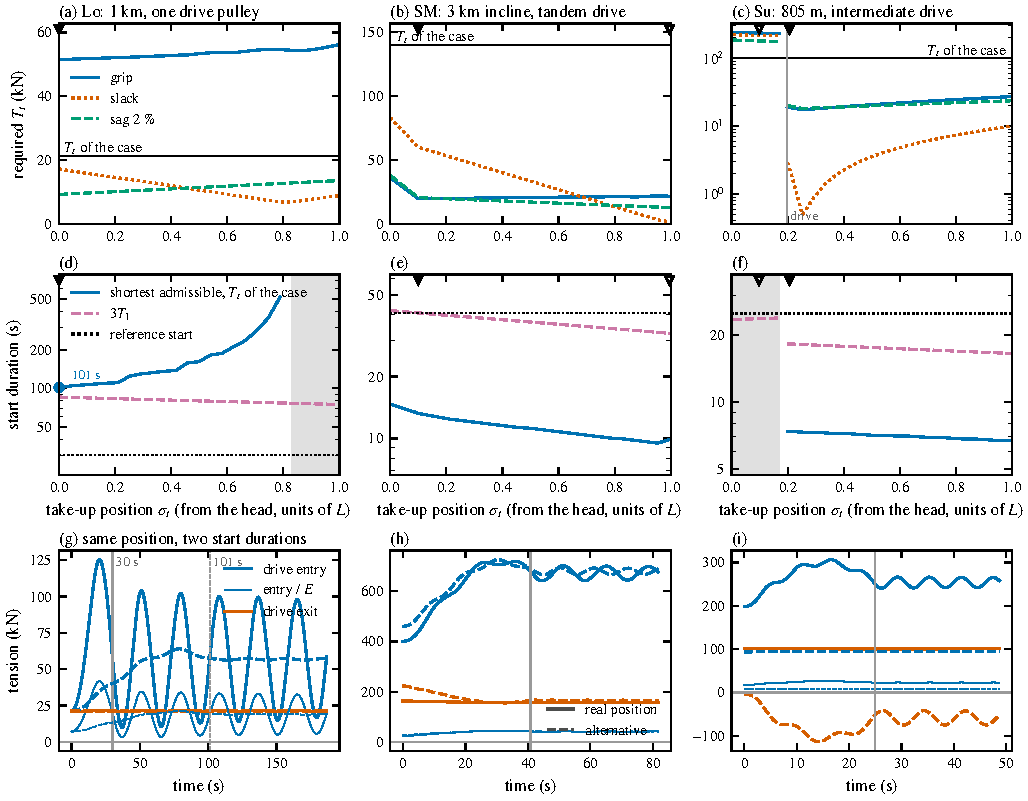
\includegraphics[width=\linewidth]{fig_applications}
  \caption{Start-ups of three conveyors from the literature in physical units, against the
  take-up position (sine profile, $\hat\zeta=0.01$, DIN~22101 strand resistances fitted to
  each $F_U$ and building up with the belt speed, gravity from each carry profile; the take-up
  is moved along the return strand with the case's counterweight). $\sigma_t$: take-up
  position from the head pulley along the return strand, in units of $L$ ($\sigma_t=\xi$ with
  a head drive). Filled triangle: real position; open triangle: alternative of the last row.
  Columns: Lo \citep{lodewijks1996}, \qty{1}{\kilo\metre}, one drive pulley
  ($\egrip=\NumLoGripFactor$), published \qty{30}{\second} start; SM
  \citep{suchorab2025longdistance}, \qty{3}{\kilo\metre} incline, tandem drive
  ($\egrip=\NumSMGripFactor$), reference start $3\tper{1}=\qty{\NumSMReferenceStart}{\second}$
  (assumed); Su \citep{surtees1995runback}, \qty{805}{\metre}, drive on the return strand at
  $\sigma_d=\NumSuDrivePos$ ($\egrip=\NumSuGripFactor$), published \qty{25}{\second} start.
  (a--c) Take-up tension required by each condition (positive tension along the loop during and
  after the start; grip; running sag below \qty{2}{\percent}), with the case's $\Tt$. (d--f)
  Shortest sine start that the case's $\Tt$ admits, with $3\tper{1}$ and the reference start;
  grey, no start is admissible (the running state already fails). (g) Lo at its real position:
  the published \qty{30}{\second} start (solid) and the shortest admissible one,
  \qty{\NumLoShortest}{\second} (dashed); grip is lost where the entry tension over $\egrip$
  (thin) exceeds the exit tension. (h) SM, real position (solid) and tail (dashed). (i) Su, real
  position (solid) and tight side of the drive (dashed), where the exit tension becomes negative.
  Values in Table~\ref{tab:applications}.}
  \label{fig:applications}
\end{figure}
% Generated by maps/paper_tables.py from maps/applications.py; do not edit by hand.
\begin{widetable}[t]
\centering
\footnotesize
\setlength{\tabcolsep}{3.5pt}
\begin{threeparttable}
\caption{Start-ups of three conveyors in physical units \citep[Lo, SM, Su:][]{lodewijks1996,suchorab2025longdistance,surtees1995runback}, real take-up position and an alternative (sine profile, $\hat\zeta=0.01$, DIN~22101 strand resistances fitted to $F_U$ and starting with the belt speed, gravity from the carry profile, the case's counterweight in every position). $\sigma_t$: take-up position from the head pulley along the return strand, in units of $L$. Peak drive-entry tension and its ratio to the running value; lowest drive-exit tension during and after the start; carriage travel; take-up tension required by the three conditions (positive tension along the loop, grip $T_\mathrm{entry}\le \mathrm{e}^{\mu\theta}T_\mathrm{exit}$, running sag below 2\,\%), the one that governs and the running exit tension it implies; shortest sine start that the case's $T_t$ admits.}
\label{tab:applications}
\begin{tabular}{@{}lrrrrrrrrrlrr@{}}
\toprule
 & & & & & \multicolumn{2}{c}{Entry peak} & Exit & & \multicolumn{3}{c}{Required} & Shortest \\
\cmidrule(lr){6-7}\cmidrule(lr){10-12}
Take-up & $\sigma_t$ & $t_1$ & $t_a$ & $t_a/t_1$ & (kN) & /running & min. & Travel & $T_t$ & governs & $T_2$ & start \\
 & & (s) & (s) & & & & (kN) & (m) & (kN) & & (kN) & (s) \\
\midrule
\multicolumn{13}{@{}l}{Lo: 1~km, one drive pulley ($\mathrm{e}^{\mu\theta}=3.0$), $T_t=21.3$~kN; published start 30~s} \\
real, 30~s & 0.001 & 28.5 & 30 & 1.05 & 125 & 2.21 & $21$ & 8.43 & 51.5 & grip & 51.5 & 101 \\
real, shortest start & 0.001 & 28.5 & 101 & 3.56 & 64 & 1.13 & $21$ & 3.20 & 21.3 & grip & 21.3 & 101 \\
tail, 30~s & 0.995 & 24.9 & 30 & 1.20 & 108 & 2.06 & $13$ & 5.15 & 56.1 & grip & 51.8 & -- \\
\midrule
\multicolumn{13}{@{}l}{SM: 3~km incline, tandem drive ($\mathrm{e}^{\mu\theta}=16.4$), $T_t=140$~kN; start $3t_1$ (assumed)} \\
real & 0.100 & 13.6 & 41 & 3.00 & 720 & 1.07 & $156$ & 0.96 & 60.0 & slack & 77.4 & 13 \\
tail & 0.995 & 10.8 & 41 & 3.77 & 726 & 1.07 & $155$ & 0.44 & 21.7 & grip & 46.9 & 10 \\
\midrule
\multicolumn{13}{@{}l}{Su: 805~m, drive at $\sigma_d=0.197$ ($\mathrm{e}^{\mu\theta}=11.5$), $T_t=100$~kN; published start 25~s} \\
real (after the drive) & 0.207 & 6.1 & 25 & 4.11 & 307 & 1.21 & $100$ & 0.25 & 19.8 & sag & 20.4 & 7 \\
tight side & 0.098 & 7.9 & 25 & 3.16 & 95 & 1.01 & $-114$ & 0.00 & 234.0 & grip & 75.2 & -- \\
\bottomrule
\end{tabular}
\begin{tablenotes}[flushleft]
\footnotesize
\item Slack: positive tension along the loop; in SM it is the weight of the return strand held from the take-up near the high end, at rest. Shortest start: --, none (the running state already fails with the case's $T_t$). The shortest start does not account for belt strength or motor torque. Su, tight side: the exit tension is negative already in running.
\end{tablenotes}
\end{threeparttable}
\end{widetable}


The formulas of Section~\ref{A-sec:results} of the article rest on idealised resistances and a
horizontal path. To see how the take-up position acts on real layouts, three conveyors of
Table~\ref{A-tab:cases} are started in physical units with the full model: a
\qty{1}{\kilo\metre} conveyor with a single drive pulley and published speed-controlled starts
\citep[\S8.6.2]{lodewijks1996}, a \qty{3}{\kilo\metre} incline with a tandem head drive
\citep{suchorab2025longdistance}, and an \qty{805}{\metre} conveyor whose drive sits on the
return strand \citep{surtees1995runback}. Resistances follow DIN~22101 strand by strand, with
the coefficient fitted to the running peripheral force of each case, and build up with the belt
speed; gravity enters through each carry profile; the start is a sine profile with the base
damping $\hat\zeta=0.01$. The take-up is moved along the whole return strand with the
counterweight of the case, so $\Tt$ and $\beta$ stay fixed. At fixed take-up mass the total
tension is $\Tt$ plus a field that does not depend on $\Tt$, so each condition of
Section~\ref{A-sec:validity} of the article gives a closed bound on $\Tt$ from a single run:
positive tension along the loop during and after the start, drive grip, and a running sag below
\qty{2}{\percent}. The last is the value used in the design calculations of
\citet{surtees1995runback}; DIN~22101 recommends less than \qty{1}{\percent} in steady
operation, mainly for energy efficiency \citep[\S8.2.3]{din22101}. The largest of the three
bounds is the required take-up tension, and the shortest admissible start is the shortest sine
start for which the case's $\Tt$ meets all three, at that duration and beyond. The condition of
the article that the take-up follows the belt (condition (i) at the take-up) never comes close: its margin is at
least \NumAppAccelMarginMin\ in all runs. Resizing the counterweight to keep the running exit
tension, instead of keeping the counterweight, changes the required tension and $\tper{1}$ by
less than \qty{0.3}{\percent}.
% tests: test_applications.py (exact superposition; slow-start limit equal to the running grip
% condition; carriage margin > 10; same-counterweight convention immaterial within 0.3 %)

\paragraph{One drive pulley: the grip sets the start time} Lodewijks' conveyor has a single
drive pulley with $\egrip=\NumLoGripFactor$ and a take-up tension of
\qty{\NumLoTt}{\kilo\newton}, which he dimensioned for grip with the start-up factor 1.2 of a
drain-type fluid coupling \citep[Table~8.2 and Eqs.~8.7--8.9]{lodewijks1996}. His
\qty{30}{\second} speed-controlled starts, linear ramps with an initial offset, last about one
fundamental period and fall in the overshoot of the universal curve: across the start profiles of his Table~8.7 the ratio of
drive-entry to drive-exit tension reaches \NumLoGripRatioMin\ to \NumLoGripRatioMax, against the
limit of \NumLoGripFactor. A sine start of the same duration would need
\qty{\NumLoTtReq}{\kilo\newton} at the take-up, \NumLoSineTtFactor\ times the installed tension,
to stay in grip; a rigid belt with the same loads would already need
\qty{\NumLoTtReqRigid}{\kilo\newton}, so the dynamics add \qty{\NumLoDynamicIncrement}{\percent}
to a requirement that the statics of the start already violate. In effect the take-up was sized
with the start-up factor of a fluid coupling and then started under speed control in about one
fundamental period. His simulations could not show this, since the drive pulleys were modelled
without slip \citep[p.~137]{lodewijks1996}. With his take-up the shortest admissible sine start
is \qty{\NumLoShortest}{\second}, \NumLoShortestOverPeriod\ periods, above the
$2$--$3\,\tper{1}$ of the design rule: with one drive pulley the grip, not the dynamic
amplification, fixes the start time. Moving the take-up away from the drive adds the resistance
of the return run to the required tension, while the required running exit tension hardly
changes (Table~\ref{tab:applications}), and beyond $\xi=\NumLoXiLimit$ the installed tension no
longer holds grip even in steady running (Fig.~\ref{fig:applications}a, d). The real position,
next to the drive, is the best one.

\paragraph{Tandem drive on an incline: the statics decide} The incline of
\citet{suchorab2025longdistance} has a tandem drive ($\egrip=\NumSMGripFactor$) and a take-up
tension of \qty{\NumSMTt}{\kilo\newton}. Its take-up sits at $\xi=0.1$, near the high end, where
at rest it must hold the weight of the return strand down the slope: this alone requires
\qty{\NumSMTtReq}{\kilo\newton}, against \qty{\NumSMTtReqTail}{\kilo\newton} with the take-up at
the tail, where grip governs, and up to \qty{\NumSMTtReqMax}{\kilo\newton} next to the drive. The
installed tension covers every position, and the start could be as short as
\qty{\NumSMShortest}{\second}, about \NumSMShortestOverPeriod\ fundamental period. Moving the
take-up to the tail shortens the fundamental period by \qty{\NumSMPeriodChange}{\percent}
(\qty{\NumLoPeriodChange}{\percent} in Lodewijks' conveyor), but changes the peak drive-entry
tension by less than one per cent (Table~\ref{tab:applications}): with a large wave-speed ratio
the carry strand dominates strand~B wherever the take-up is.

\paragraph{Drive on the return strand: the tight side} Surtees' conveyor has its drive at
$\sigma_d=\NumSuDrivePos$ from the head and the take-up right after it, on the slack side. There
the running sag governs and requires \qty{\NumSuTtReq}{\kilo\newton}, close to the lowest value
along the slack side (\qty{\NumSuTtReqBest}{\kilo\newton}); the installed
\qty{100}{\kilo\newton} admits starts from \qty{\NumSuShortest}{\second}, about
\NumSuShortestOverPeriod\ fundamental periods. On the tight side of the drive the take-up would
need \qty{\NumSuTtReqTight}{\kilo\newton}, \NumSuTightFactor\ times more: with the installed
counterweight the exit tension is negative already in running and falls to
\qty{\NumSuExitTight}{\kilo\newton} during the start (Fig.~\ref{fig:applications}i). The
impractical region of \ref{A-app:validity} of the article appears on a real layout.

\paragraph{What the take-up position does on real conveyors} In these three conveyors the take-up
position acts mainly through the statics: through the resistance of the return run between the
drive and the take-up, and through the weight of the return strand on a slope. Its dynamic
effect, a fundamental period that changes by \NumLoPeriodChange\ to
\qty{\NumSMPeriodChange}{\percent} between the real position and the tail in Lo and SM, enters
through the start time. With one drive pulley the grip fixes the start time; with a tandem drive or a
generous take-up tension the limits come from the belt strength and the motor, which this
analysis does not evaluate.

% =====================================================================
% Supplementary material, S3 -- drive on the return strand and initial crawl.
% Numbers: paper_numbers.py (NC*, Intermediate*, Crawl* macros).
% Tests: test_intermediate.py (three-segment equation vs an independent
% implementation, both sides, bounds, reversal of travel,
% test_startup_collapse_intermediate: +4.5 %, +2.5 %); test_metrics.py (crawl:
% ramp of one period removes the resistance overshoot).
% =====================================================================
\section{Drive on the return strand and initial crawl}\label{supp:intermediate}

\paragraph{Drive on the return strand} With the drive at $\sigma_d$ on the return strand and the
take-up downstream of it, strand~B runs from the take-up through a return run $\ell_2$ to the
tail, the whole carry strand, and a return run $\ell_1=\sigma_d/L$ from the head to the drive;
strand~A is the uniform return run between the drive and the take-up. With the take-up as a free
end, the frequencies of strand~B follow from
\begin{equation}\label{eq:strandB3}
  \gamma\tan\Omega\ell_1\,\tan\gamma\Omega+\tan\Omega\ell_1\,\tan\Omega\ell_2
  +\frac{1}{\gamma}\tan\Omega\ell_2\,\tan\gamma\Omega=1,
\end{equation}
which reduces to Eq.~(\ref{A-eq:strandB}) of the article for $\ell_1=0$, to
$\tan\Omega\ell_1\tan\gamma\Omega=1/\gamma$ for a take-up at the tail ($\ell_2=0$), and, for
$\gamma=1$, to $\Omega(\ell_1+1+\ell_2)=\pi/2$ by the tangent addition formula. Strand~B again
holds the fundamental for $\gamma\ge1$ and any position of the drive and take-up on the return
strand: by Rayleigh's principle, adding belt at either end of the carry strand lowers its
frequency, so $\Omega_{B1}\le\pi/(2\gamma)\le\pi/2<\Omega_{A1}$. A take-up upstream of the
drive, on its tight side, gives the same family with the roles of $\ell_1$ and $\ell_2$
exchanged, since reversing the direction of travel leaves the spectrum unchanged; that position
is impractical for other reasons (\ref{A-app:validity} of the article). The period
bounds become
\begin{equation}\label{eq:bounds_intermediate}
  4\gamma<\tauper{1}\le4\tauB+4(\gamma-1)\,\ell_1,\qquad \tauB=\gamma+\ell_1+\ell_2,
\end{equation}
where the upper bound follows from giving the run $\ell_1$ the density of the carry strand,
which can only lengthen the period, and applying Eq.~(\ref{A-eq:bounds_head}) of the article. The
run $\ell_1$ sits at the fixed end of the heavy strand and acts as a soft spring: the period now
exceeds four transits, by up to \qty{\NumIntermediateOverMax}{\percent} for $\gamma=3$
(Fig.~\ref{A-fig:modal}d of the article), and the rule of four transits errs in opposite
directions with a head and with an intermediate drive. For $\gamma=1$ only the total length of
the strand matters. On the geometry of \citet{nordell1984}, with the drive \qty{5150}{ft} from
the head and the take-up \qty{300}{ft} downstream of it, the fundamental period is
\qty{\NumNCPeriod}{\second} against four transits of \qty{\NumNCFourTransit}{\second}
($\tauper{1}/(4\tauB)=\NumNCRatio$); with a head drive and the same strand lengths it would be
\qty{\NumNCPeriodHead}{\second} ($\NumNCRatioHead$), so the position of the drive alone
lengthens the period by \qty{\NumNCIncrease}{\percent}. Since the modes of a strand share out
its mass, the effective mass of the fundamental never exceeds $m_B$. Moving the drive away from
the head thus lengthens $\tper{1}$ and calls for slower starts at the same dynamic amplification.
With the drive on the return strand, strand~A is still uniform and the exit formula of
Eq.~(\ref{A-eq:startup_formulas}) of the article remains exact; the entry peak lies slightly above
the universal curve, by at most \qty{4.5}{\percent} for $\tau_a=\tauper{1}$ and
\qty{2.5}{\percent} for $2\tauper{1}$ with the drive within $0.2L$ of the head.

\paragraph{Initial crawl} Practice often starts with a crawl at low speed: a ramp to
\qty{4}{\percent} of the speed in \qty{20}{\second} held for \qty{60}{\second} at ZISCO
\citep{nordell1997zisco}, and a plateau of \qty{60}{\second} at \qty{10}{\percent} added at
Henderson so that the take-up could keep pace with the belt stretch \citep{kung2005henderson}.
For a uniform strand with resistances of Coulomb type, which appear in full once the belt moves
($\rho=1$ and 5, $\zeta_1=0.01$ and $0.1$), and a crawl at \qty{5}{\percent} of the final speed
before a parabolic acceleration of three periods, the effective part is the ramp to crawl
speed. The peak at the fixed end, over the running-plus-inertial force, is
\NumCrawlAbruptMin--\NumCrawlAbruptMax\ with an abrupt onset,
\NumCrawlRampHalfMin--\NumCrawlRampHalfMax\ with a ramp of half a period and
\NumCrawlRampOneMin--\NumCrawlRampOneMax\ with a ramp of one period $\tper{s}$, which lasts an
odd number of periods of every mode of the strand and so leaves the resistance load without
residual oscillation; the take-up travel falls from
\NumCrawlTravelAbruptMin--\NumCrawlTravelAbruptMax\ times its quasi-static value to at most
\NumCrawlTravelRampOneMax. A hold at crawl speed barely helps with light damping, because the
first overshoot of the resistances occurs during the hold; with $\zeta_1=0.1$ it lets the
transient decay, from \NumCrawlHoldDampedZero\ to \NumCrawlHoldDampedOne\ and
\NumCrawlHoldDampedTwo\ after one and two periods. With speed control, a ramp to crawl speed of
at least one period does the work. Since the resistances appear along the whole loop at once in
the model, while in a real start they follow the stretch front, the abrupt onset is an upper
bound.

% =====================================================================
% S4 -- Parameters of the illustrative conveyors of the verification (Fig. 2 of the
% article). Source: validation/fig_lumped_validation.py (CASES, conveyor()).
% =====================================================================
\section{Illustrative conveyors of the verification}\label{sec:supp_lumped}

The two conveyors of Fig.~\ref{A-fig:validation} of the article share the belt and the loads:
$L=\qty{3000}{\metre}$, $EA=\qty{120}{\mega\newton}$, inertial line densities
$\mu_r=40$ and $\mu_c=\qty{100}{\kilo\gram\per\metre}$ (weighing densities 30 and
\qty{80}{\kilo\gram\per\metre}), a counterweight hung directly on two strands with
$\Tt=\qty{70}{\kilo\newton}$, resistances $r_r=15$ and $r_c=\qty{45}{\newton\per\metre}$ with
onset $\varphi=V/V_\infty$, Kelvin--Voigt time $t_v=\qty{0.3}{\second}$, and a start to
$V_\infty=\qty{5}{\metre\per\second}$ in $t_a=\qty{60}{\second}$.
\begin{itemize}
  \item Conveyor~V1: head drive, take-up \qty{60}{\metre} downstream of it; the carry strand rises
  \qty{10}{\metre} over the first \qty{1500}{\metre} from the tail and \qty{30}{\metre} over the
  rest; sine profile.
  \item Conveyor~V2: drive on the return strand \qty{1200}{\metre} from the head, take-up
  \qty{300}{\metre} downstream of it ($\xi=0.1$); horizontal; parabolic profile.
\end{itemize}
The modal solution uses 120 modes; the lumped model, $N$ elements and the Newmark scheme with a
time step of $12.5/N$~s.

% =====================================================================
% Supplementary material, S5 -- further details of Sections 3-5 and Appendix C.
% Moved from the article in the cut of the second independent review (paso 7.5d).
% Numbers: paper_numbers.py (StepOvershootEntry, BetaFiveAOneSlope, AOneStartRatioMin,
% WR*, Harrison* macros). Tests: test_response.py::test_step_overshoot_can_exceed_two
% (2.18, confirmed with FE); test_beta_min.py; test_harrison.py.
% Sources checked: wheatley2021 (Table 1, conveyors B and C); harrison1985b (Sect. 3:
% rotor resistance switched out in steps); song2012 (text p. 220 against Tables 1-2,
% p. 221; travel 2.81 m in Sect. 3.1 and 2.85 m in Sect. 3.3 and Table 2).
% =====================================================================
\section{Further details}\label{supp:details}

\paragraph{Step onset of the resistances (Section~\ref{A-sec:modal})} With a unit step $\varphi$
each mode overshoots its quasi-static response by a factor two, but the tension field is not
bounded by that factor: with $\gamma=2$, $\beta=0.1$, $\xi=0.05$ and resistances uniform per unit
length, the undamped peak at the drive entry reaches \NumStepOvershootEntry\ times the
quasi-static value (full loop, 300 modes).

\paragraph{Threshold of the mode A1 (Section~\ref{A-sec:betaregime})} The mode A1, the
quarter-wave mode of strand~A, has a small threshold, $\betafive\simeq\NumBetaFiveAOneSlope\,\xi$,
but a short period, $4\xi L/c_r$: even with the take-up at the tail the published starts of the
conveyors of Table~\ref{A-tab:cases} last about \NumAOneStartRatioMin\ of its periods or more (the
least, Lo), so
they drive it quasi-statically.

\paragraph{Short conveyors (Section~\ref{A-sec:betaregime})} The \qty{275}{\metre} conveyor of
\citet{wheatley2021} (WR) reaches its threshold only at the weakest coupling of its material
($\beta/\betafive=\NumWRRatioLowMin$--$\NumWRRatioLowMax$). Of the other conveyors of the same
plant \citep[Table~1]{wheatley2021}, with a counterweight hung directly on two strands and the
take-up position of WR assumed, the \qty{\NumWRBLength}{\metre} conveyor~B gives
$\beta/\betafive=\NumWRBRatio$, and only the \qty{\NumWRCLength}{\metre} conveyor~C lies clearly
beyond its threshold ($\beta/\betafive=\NumWRCRatio$); there the exact
equation~(\ref{A-eq:chareq}) keeps the mass.

\paragraph{The drive of Harrison's conveyor (Section~\ref{A-sec:fieldchecks})} The slow period of
the model exceeds Harrison's by \qty{\NumHarrisonSlowExcess}{\percent}, and the record shows an
elastic ripple of \qty{\NumHarrisonWaveMeas}{\second} in our read-out of
\citet[Fig.~5c]{harrison1983}, which the model with prescribed velocity does not have (its second
period is \NumHarrisonSecondMin--\qty{\NumHarrisonSecondMax}{\second}). Both point to the drive:
three wound-rotor motors started by torque steps. Equation~(\ref{A-eq:chareq_torque}) tests this
with the reduced drive mass $m_d$ and the slip dashpot $\hat c$ of \ref{A-app:torque},
neither of which is published:
\begin{itemize}
  \item A free drive ($m_d\to0$, $\hat c=0$) gives periods of
  \qty{\NumHarrisonFreeDriveSlow}{\second} and \qty{\NumHarrisonFreeDriveSecond}{\second}: with
  the take-up next to the drive the loop vibrates as a free--free string of length $2L$, and its
  second period is the loop transit, close to the measured ripple.
  \item Drive inertia alone reaches the measured slow period with $m_d=\NumHarrisonDriveMassMeas$,
  a reduced drive mass \NumHarrisonDriveMassBeltRatio\ times that of the whole belt, and then gives
  \qty{\NumHarrisonDriveMassSecond}{\second} for the second period.
  \item A linearised slip characteristic, $c_d=F/(sV)$ with the running force
  $F=\qty{\NumHarrisonRunForce}{\kilo\newton}$ (\qty{900}{\kilo\watt} at
  \qty{3.7}{\metre\per\second}), gives $\hat c\approx\NumHarrisonDashpotNatural$ for a slip of
  \qty{\NumHarrisonSlipNatural}{\percent}, typical of a motor with the rotor short-circuited. The
  slow period then changes by at most \qty{\NumHarrisonDashpotNaturalChange}{\percent} for
  $\NumHarrisonDriveMassMin\le m_d\le\NumHarrisonDriveMassMax$: the drive acts as a prescribed
  velocity. With rotor resistance in circuit, slips of
  \NumHarrisonSlipSoftMin--\qty{\NumHarrisonSlipSoftMax}{\percent} give
  $\hat c\approx\NumHarrisonDashpotSoftMin$--$\NumHarrisonDashpotSoftMax$, and with $m_d=1$--$3$
  the slow period falls to \NumHarrisonSoftSlowMin--\qty{\NumHarrisonSoftSlowMax}{\second}, with
  damping ratios of \NumHarrisonSoftZetaMin--\NumHarrisonSoftZetaMax\ and a second period of
  \NumHarrisonSoftSecondMin--\qty{\NumHarrisonSoftSecondMax}{\second}.
\end{itemize}
No single linear drive reproduces both features: the ripple requires a nearly free drive, and the
slow period a soft slip characteristic or a heavy drive. A drive whose characteristic changes
during the start would produce both, and these motors had their rotor resistance switched out in
steps as the speed rose \citep[Sect.~3]{harrison1985b}.

\paragraph{The stored belt of Harrison's conveyor (Section~\ref{A-sec:fieldchecks})}
\Citet{harrison1985b} reports that the take-up loop supplied \qty{\NumHarrisonStoredMeas}{\metre}
of belt at start-up. The start check of Section~\ref{A-sec:fieldchecks} stores at most
\qty{\NumHarrisonStoredMax}{\metre}, but it applies only the inertial load of the first plateau.
The stored belt is a quasi-static quantity, set by the running tensions and the stiffness of the
belt rather than by the dynamics: the running resistances alone add
\NumHarrisonStoredRunMin--\qty{\NumHarrisonStoredRunMax}{\metre} if the whole force of the
installed \qty{900}{\kilo\watt} acts on the empty belt ($\mu_r=81$ or
\qty{40}{\kilo\gram\per\metre}, the two densities that his data allow). Since neither the running
tensions of the empty belt nor its stiffness are published, the stored belt does not test the
take-up model; its order of magnitude is consistent with the record.

\paragraph{Inconsistencies in the example of Song et al. (\ref{A-app:validation})}
Besides the take-up tension and travel discussed in the article, the text and the tables of
\citet{song2012} disagree: the steady take-up travel is \qty{2.81}{\metre} in their \S3.1 and
\qty{2.85}{\metre} in their \S3.3 and Table~2, the maximum travel \qty{3.37}{\metre} in the text
and \qty{3.72}{\metre} in Table~2, and the steady drive tensions 337 and \qty{113}{\kilo\newton} in
the text and 309 and \qty{37}{\kilo\newton} in their Table~1.


\bibliographystyle{elsarticle-num-names}
\bibliography{references}

\end{document}
